% Physics tree regression derived from TikZ missing-child semantics.
\documentclass[border=2pt]{standalone}
\usepackage{tikz}
\usetikzlibrary{trees}

\begin{document}
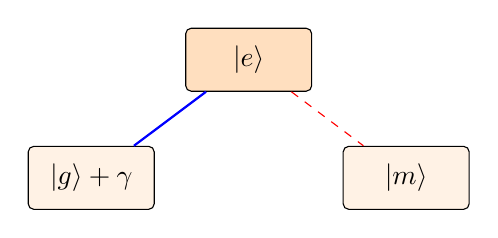
\begin{tikzpicture}[
  grow=down,
  level distance=15mm,
  sibling distance=20mm,
  every node/.style={draw,rectangle,rounded corners=2pt,minimum width=16mm,minimum height=8mm,fill=orange!10}
]
  \node[fill=orange!25] {$|e\rangle$}
    child {node {$|g\rangle+\gamma$} edge from parent[blue,thick]}
    child[missing] {node {$|u\rangle$}
      child {node {unobserved}}
    }
    child {node {$|m\rangle$} edge from parent[red,dashed]};
\end{tikzpicture}
\end{document}
